\section{Техническое задание}
\subsection{Основание для разработки}

Основанием для разработки является задание на выпускную квалификационную работу бакалавра "<Программная система визуализации трехмерных данных, использующая библиотеку OpenGL">.

\subsection{Цель и назначение разработки}

Основной задачей выпускной квалификационной работы является разработка программной системы для визуализации трёхмерных данных, использующая библиотеку OpenGL.

Используя библиотеку OpenGL последней версии, планируется разработать приложение на языке C\#, способное импортировать и обрабатывать массивы трёхмерных данных и в дальнейшем визуализировать их в виде трёхмерных моделей.

Задачами данной разработки являются:
\begin{itemize}
\item разработка и проектирование основы графического движка;
\item реализация программы парсеров, способных обрабатывать, преобразовывать и загружать в программу трёхмерные данные;
\item разработка и реализация функции хранения трёхмерных данных внутри программы и их загрузки из внешней файловой среды;
\item разработка интерфейса для взаимодействия с программой;
\item создание готовой программы, реализующей графику, на основе спецификации и библиотеки OpenGL.
\end{itemize}

\subsection{Требования к программной системе}

\subsubsection{Требования к данным программно-информационной системы}

Входными данными для программной системы являются файлы с расширением *.obj, внутри которых содержится информация в виде массивов трёхмерных данных; файлы текстур - изображения с расширением *.png и *.jpg; данные ввода с клавиатуры и мыши, которые служат для управления перемещением и вращением камеры.

Выходными данными для программной системы являются файлы данных, содержащие информацию о загруженных объектах и ресурсах в программную среду, а также выводимое на экран изображение двумерной проекции трёхмерных объектов на виртуальной сцене.

На рисунке ~\ref{diagram1:image} представлена диаграмма описания потоков данных в программе.

\begin{figure}[ht]
	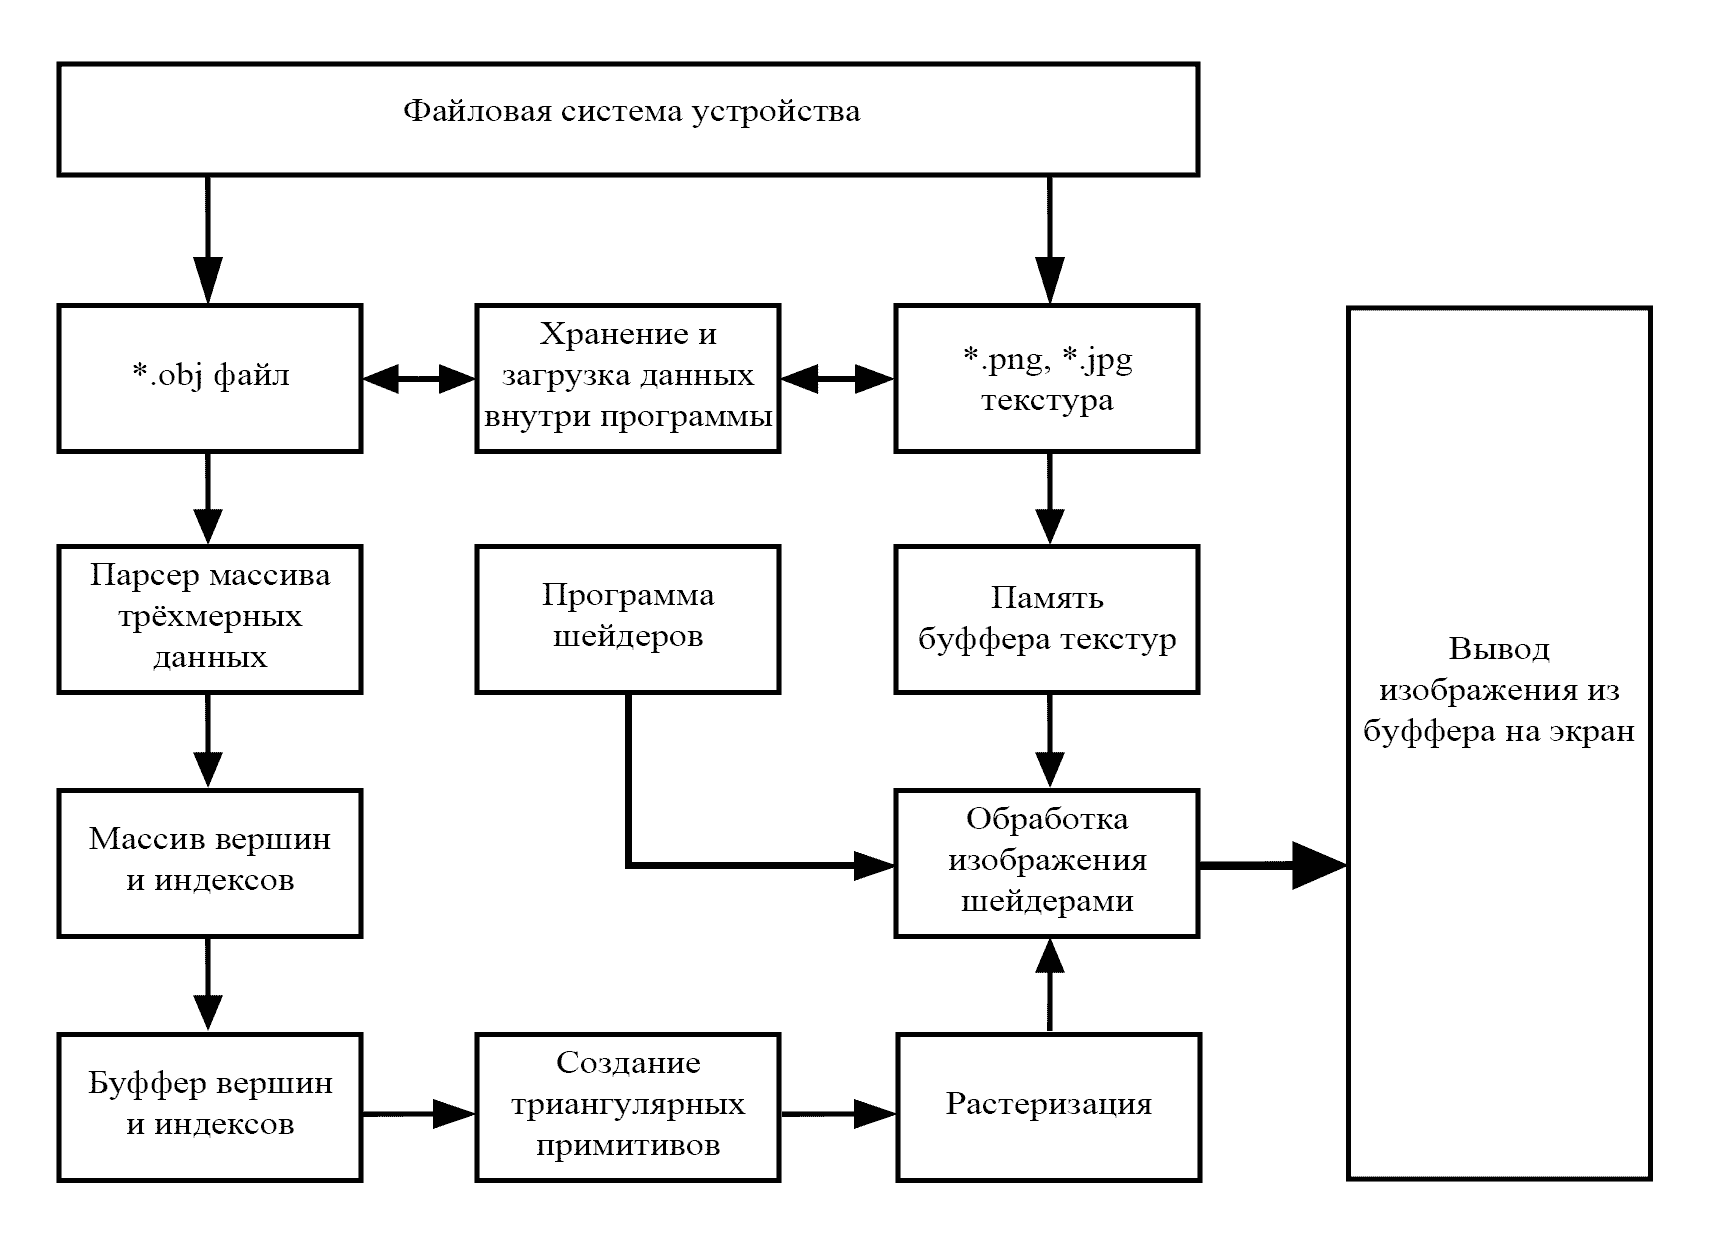
\includegraphics[width=1\linewidth]{diagram1.png}
	\caption{Диаграмма потоков данных в программе}
	\label{diagram1:image}
\end{figure}

\subsubsection{Функциональные требования к программной системе}

Программа должна реализовывать следующие функции:
\begin{itemize}
    \item позволять пользователю импортировать любые массивы трёхмерных данных (включая текстуры для трёхмерных моделей);
    \item выполнять отрисовку трёхмерной сцены в реальном времени (каждый кадр);
    \item пользволять пользователю свободно управлять перспективой виртуальной камеры;
    \item предоставлять возможность преобразовывать массив трёхмерных данных (производить аффинные преобразования) в рамках: сдвига, вращения и растяжения (сжатия);
    \item предоставлять возможность управлять настройками освещения - источником света (прямой свет, отраженный свет и рассеянный свет);
    \item импортировать, хранить и загружать массив трёхмерных данных внутри самой программы.
\end{itemize}

Виды преобразований массива трёхмерных данных, предоставляемых программой, представлены на рисунке ~\ref{affin:image}.

\begin{figure}[ht]
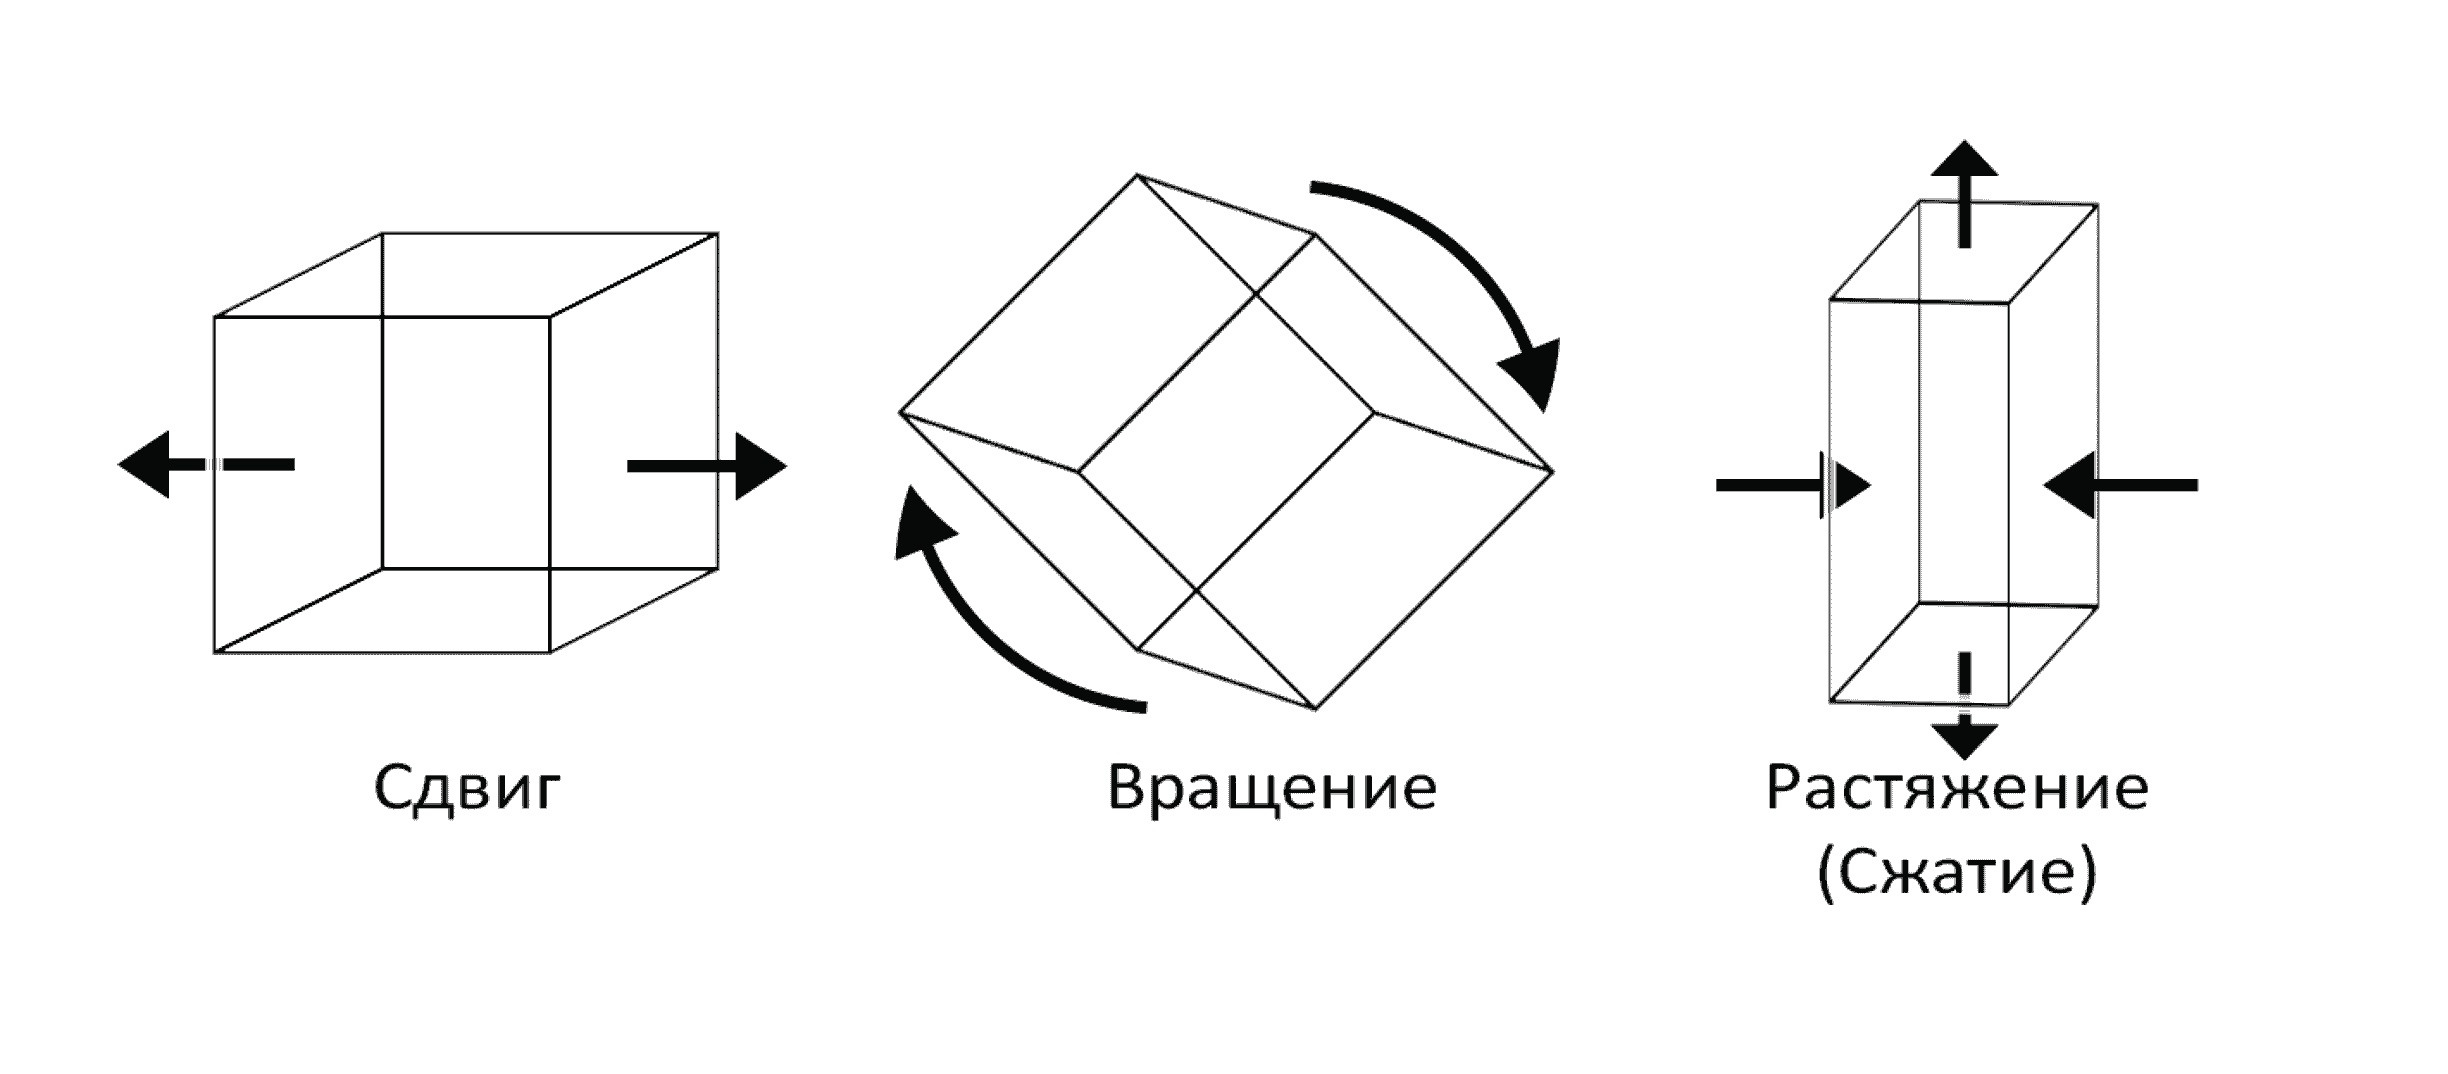
\includegraphics[width=1\linewidth]{affin.png}
\caption{Виды преобразований массива трёхмерных данных}
\label{affin:image}
\end{figure}
%\vspace{-\figureaboveskip} % двойной отступ не нужен (можно использовать, если раздел заканчивается картинкой)

Виды света, реализуемые программной системой, чьи настройки атрибутов предоставляются программной системой пользователю, представлены на рисунке ~\ref{diagram8:image}.

\begin{figure}[ht]
	\center{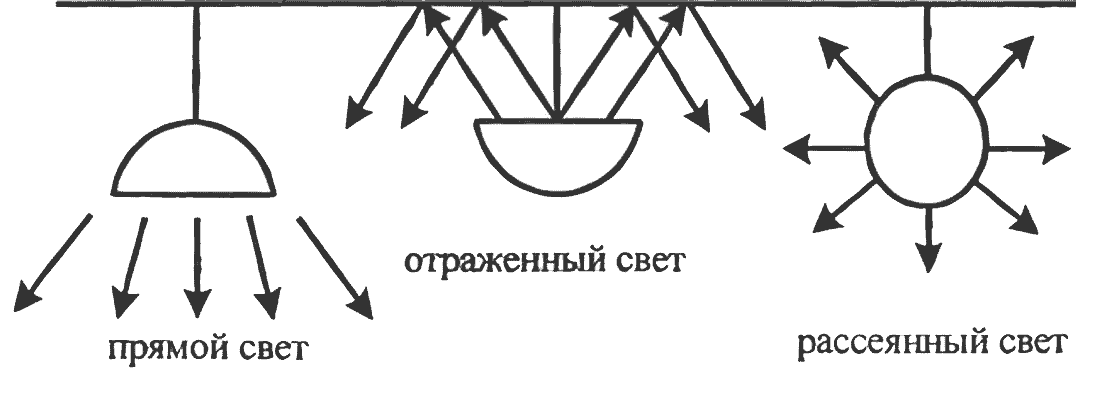
\includegraphics[width=0.8\linewidth]{diagram8.png}}
	\caption{Виды света, излучаемые источником освещения}
	\label{diagram8:image}
\end{figure}

\subsubsection{Требования к графическому интерфейсу программы}

Программное обеспечение должно иметь содержательный и интуитивно понятный интерфейс. Большую часть основного окна приложения должно занимать само окно вывода растрового изображения проекции виртуальной сцены и всех трёхмерных данных, загруженных в программу. Сбоку, поверх основного окна приложения должно находиться специально выведенное отдельное окно «инспектора», с помощью которого пользователь сможет управлять загрузкой и сохранением массивов трёхмерных данных, а также взаимодействовать с уже существующими данными на виртуальной сцене.

Макет пользовательского интерфейса, составленный по данным требованиям представлен на рисунке ~\ref{maket1:image}

\begin{figure}[H]
	\center{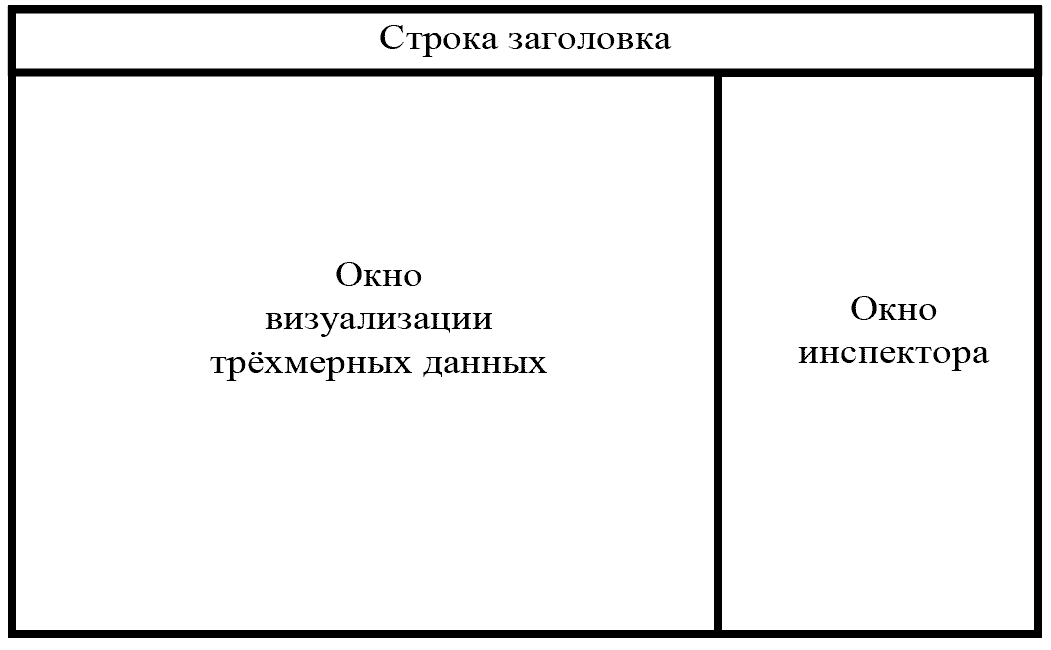
\includegraphics[width=0.85\linewidth]{maket1.png}}
	\caption{Макет пользовательского интерфейса}
	\label{maket1:image}
\end{figure}

\subsection{Моделирование вариантов использования}

Для разрабатываемого программного обеспечения была реализована модель, которая демонстрирует наглядное представление вариантов использования программы.

На основании анализа предметной области в программе должны быть реализованы следующие прецеденты:
\begin{enumerate}
\item Импортирование массивов трёхмерных данных из файловой системы пользователя.
\item Просмотр визуализированного массива трёхмерных данных в виде отрисованных объектов на экране.
\item Осуществление трансформаций над массивом трёхмерных данных.
\item Настройка параметров источника света и общего освещения.
\item Хранение, загрузка и удаление массивов трёхмерных данных из программной системы.
\end{enumerate}

На рисунке ~\ref{diagram2:image} представлена диаграмма вариантов использования

\begin{figure}[H]
	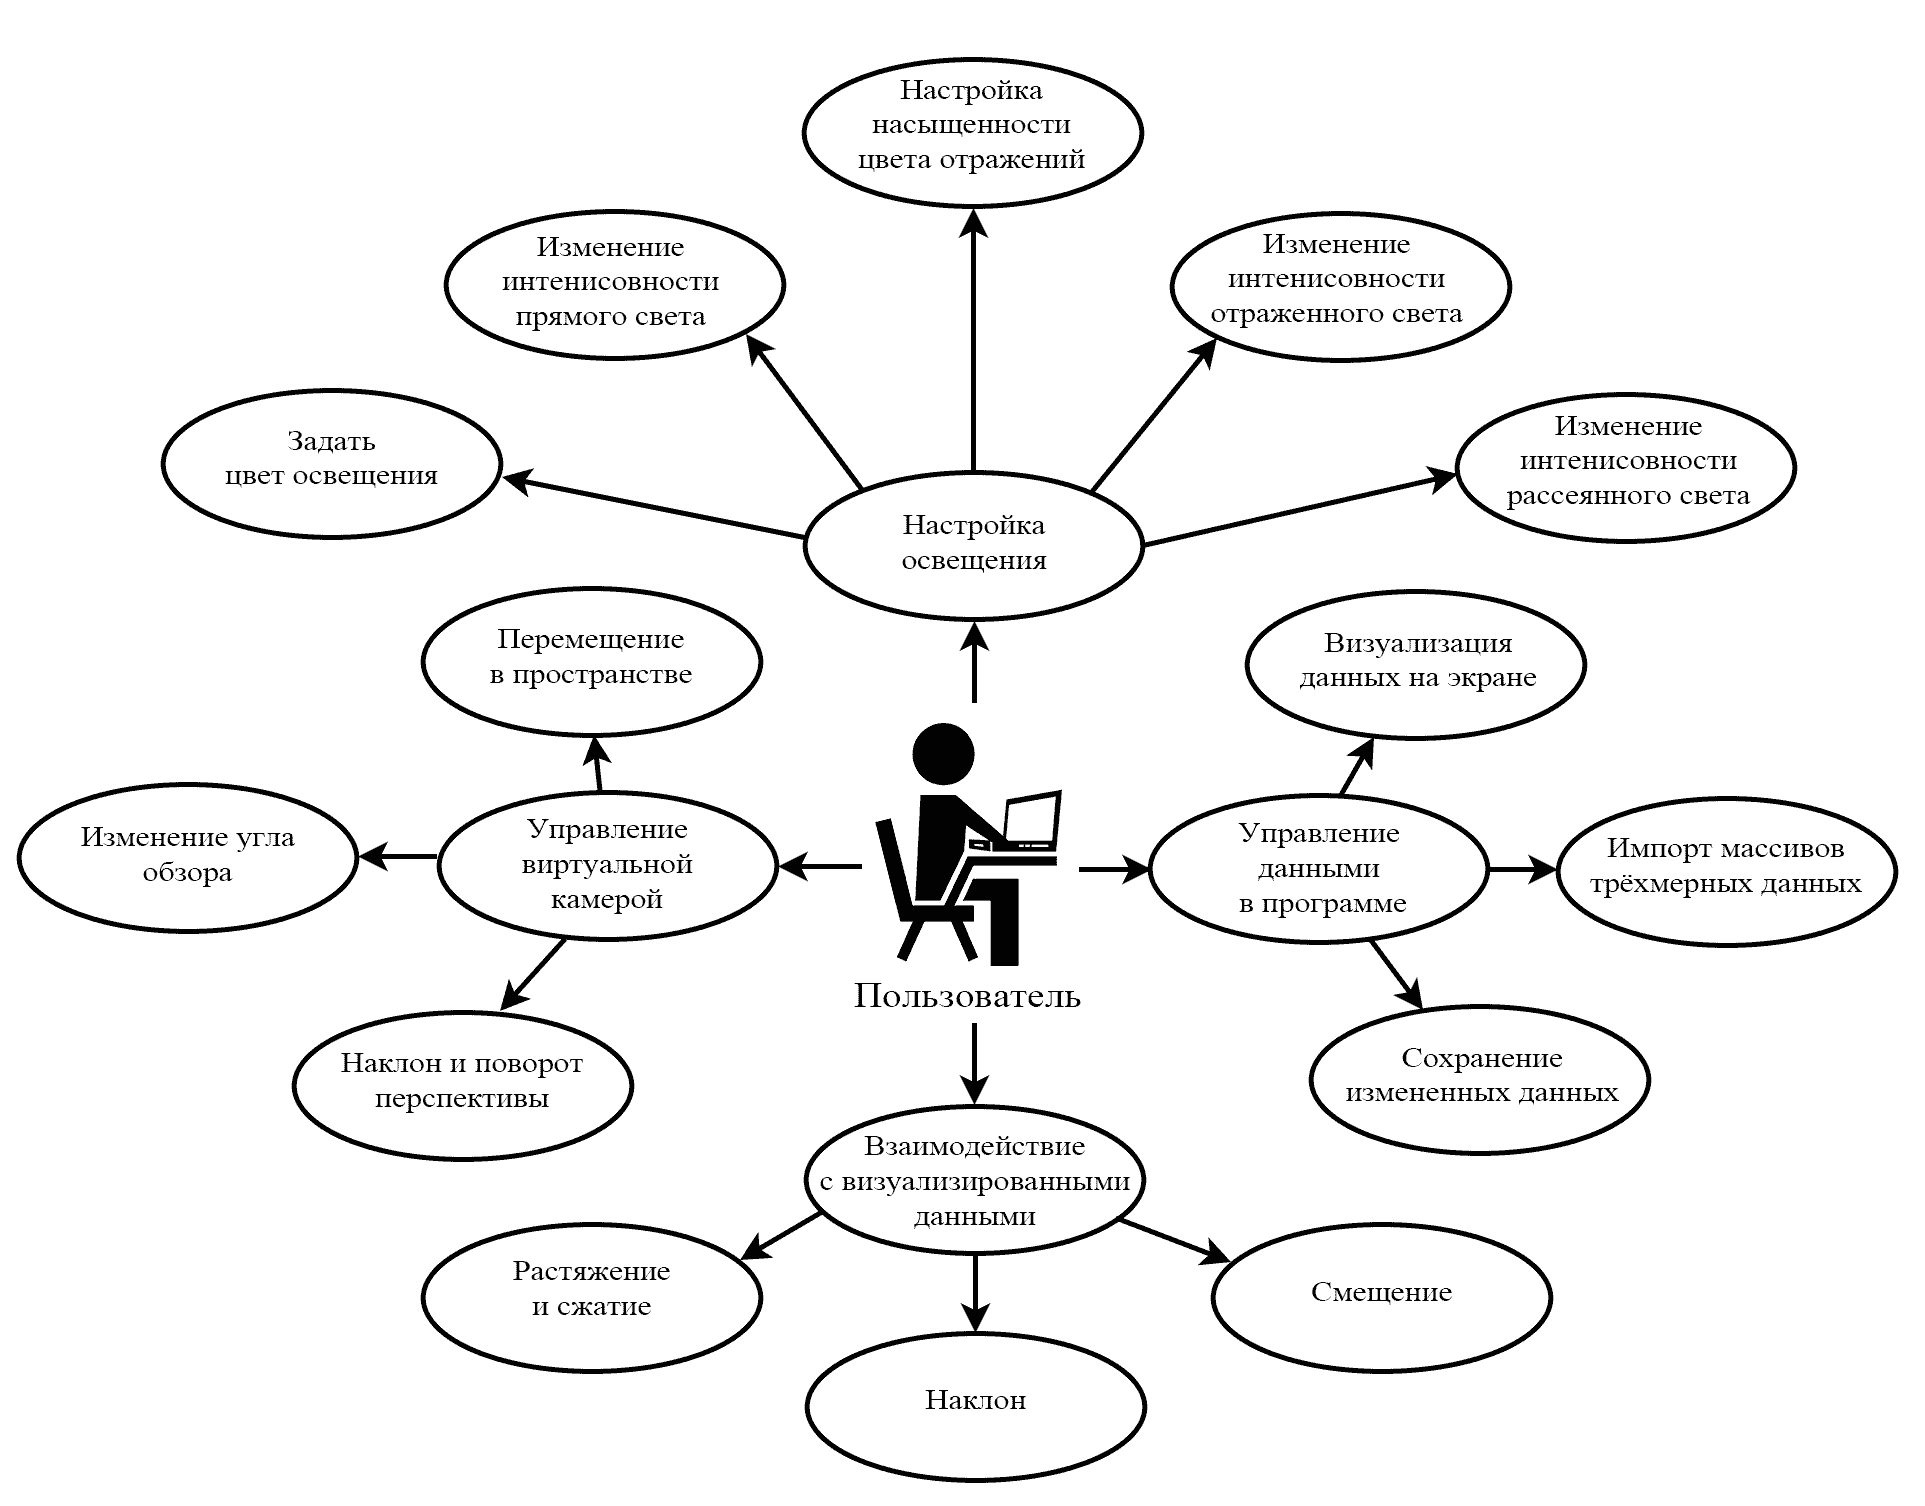
\includegraphics[width=1.06\linewidth]{diagram2.png}
	\caption{Диаграмма вариантов использования}
	\label{diagram2:image}
\end{figure}

На данном рисунке представлена диаграмма, которая в общих чертах описывает модель вариантов использования программы. При взаимодействии с программой, пользователь будет осуществлять одно или сразу несколько действий из представленной модели вариантов использования. Для моделирования  более конкретных случаев работы программы, было написано несколько сценариев вариантов использования.

\subsubsection{Вариант использования: Визуализация данных на экране}

Результат варианта использования: пользователь, выбрав из списка необходимый объект, загружает его на виртуальную сцену и наблюдает скомпилированную композицию трёхмерной сцены с объектом на ней в основном окне программы.

Сценарий использования описан в таблице \ref{table:scene3}

\begin{xltabular}{\textwidth}{|X|p{3.5cm}|>{\setlength{\baselineskip}{0.7\baselineskip}}p{9.85cm}|>{\setlength{\baselineskip}{0.7\baselineskip}}p{4.85cm}|}
	\caption{Сценарий варианта использования: Визуализация данных на экране.\label{table:scene3}}\\
	\hline \centrow \setlength{\baselineskip}{0.7\baselineskip} Номер шага & \centrow \setlength{\baselineskip}{0.7\baselineskip} Действующее лицо & \centrow Действие \\\hline
	\endfirsthead
	\finishhead
	\hline \centrow 1 & \centrow Пользователь & Пользователь, находясь во вкладке инспектора "<Объект">, нажимает на выпадающее меню напротив надписи "<Объект">.\\
	
	\hline \centrow 2 & \centrow Система & Появляется список выпадающего меню, содержащий наименования всех хранящихся трёхмерных объектов в программе.\\
	
	\hline \centrow 3 & \centrow Пользователь & Пользователь кликает на строку с желаемым именем объекта в списке\\
	
	\hline \centrow 4 & \centrow Пользователь & Пользователь нажимает на кнопку "<Загрузить">.\\
	
	\hline \centrow 5 & \centrow Система & На экране пользователя отображается композиция трёхмерной сцены, на которой будет отображен выбранный раннее пользователем объект, а также источник освещения.\\
\end{xltabular}

\subsubsection{Вариант использования: Преобразование модели объекта}

Результат варианта использования: пользователь, введя коэффициенты в соответствующие поля и подтвердив действия нажатием на кнопку, применяет аффиные преобразования к трёхмерной модели объекта всех трёх видов: смещение, наклон и сжатие, в результате чего трёхмерная модель объекта, находящегося на сцене, видоизменяется в соответствии с введёными значениями преобразования.

Сценарий использования описан в таблице \ref{table:scene1}.

\begin{xltabular}{\textwidth}{|X|p{3.5cm}|>{\setlength{\baselineskip}{0.7\baselineskip}}p{9.85cm}|>{\setlength{\baselineskip}{0.7\baselineskip}}p{4.85cm}|}
	\caption{Сценарий варианта использования: Преобразование модели объекта.\label{table:scene1}}\\
	\hline \centrow \setlength{\baselineskip}{0.7\baselineskip} Номер шага & \centrow \setlength{\baselineskip}{0.7\baselineskip} Действующее лицо & \centrow Действие \\\hline
	\endfirsthead
	\finishhead
	\hline \centrow 1 & \centrow Пользователь & Пользователь, находясь во вкладке инспектора "<Объект">, нажимает на выпадающее меню напротив надписи "<Объект">.\\

	\hline \centrow 2 & \centrow Система & Появляется список выпадающего меню, содержащий наименования всех хранящихся трёхмерных объектов в программе.\\

	\hline \centrow 3 & \centrow Пользователь & Пользователь кликает на строку с желаемым именем объекта в списке\\

	\hline \centrow 4 & \centrow Пользователь & Пользователь нажимает на кнопку "<Загрузить">.\\

	\hline \centrow 5 & \centrow Система & На экране пользователя отображается композиция трёхмерной сцены, на которой будет отображен выбранный раннее пользователем объект, а также источник освещения.\\
	
	\hline \centrow 6 & \centrow Пользователь & Пользователь переключается на соседнюю вкладку инспектора с названием "<Инспектор"> нажатием на соответствующую кнопку на вкладке инспектора. Далее пользователь вводит желаемые значения коэффициентов аффинных преобразований в группы ввода строк под соответстующими метками "<Позиция">, "<"Наклон">, "<Сдвиг"> и нажимает на кнопку "<Применить">\\
	
	\hline \centrow 7 & \centrow Система & К объекту, визуализированному на экране применились аффинные преобразования, с указанными пользователем коэффициентами
\end{xltabular}

\subsubsection{Вариант использования: Создание нового объекта}

Результат варианта использования: пользователь, введя имя нового объекта, и выбрав из двух выпадающих списков необходимые модель и текстуру для объекта, создаёт новый объект, имеющий указанное имя, модель и текстуру, который теперь хранится в программе и может будет в дальнейшем загружен на виртуальную сцену.

Сценарий использования описан в таблице \ref{table:scene3}

\begin{xltabular}{\textwidth}{|X|p{3.5cm}|>{\setlength{\baselineskip}{0.7\baselineskip}}p{9.85cm}|>{\setlength{\baselineskip}{0.7\baselineskip}}p{4.85cm}|}
	\caption{Сценарий варианта использования: Визуализация данных на экране.\label{table:scene3}}\\
	\hline \centrow \setlength{\baselineskip}{0.7\baselineskip} Номер шага & \centrow \setlength{\baselineskip}{0.7\baselineskip} Действующее лицо & \centrow Действие \\\hline
	\endfirsthead
	\finishhead
	\hline \centrow 1 & \centrow Пользователь & Пользователь, находясь во вкладке инспектора "<Объект">, вводит желаемое имя для объекта в строку ввода, напротив надписи "<Имя объекта">.\\
	
	\hline \centrow 2 & \centrow Пользователь & Пользователь, нажимает на выпадающее меню напротив надписи "<Модель объекта">.\\
	
	\hline \centrow 3 & \centrow Система & Появляется список выпадающего меню, содержащий названия всех  файлов трёхмерных моделей формата .obj.\\
	
	\hline \centrow 4 & \centrow Пользователь & Пользователь кликает на строку с желаемым файлом трёхмерной модели.\\
	
	\hline \centrow 5 & \centrow Пользователь & Пользователь, нажимает на выпадающее меню напротив надписи "<Текстура объекта">.\\
	
	\hline \centrow 6 & \centrow Система & Появляется список выпадающего меню, содержащий названия всех  файлов изображений текстур формата .png и .jpg.\\
	
	\hline \centrow 7 & \centrow Пользователь & Пользователь кликает на строку с желаемым файлом изображения текстуры.\\
	
	\hline \centrow 8 & \centrow Пользователь & Пользователь нажимает на кнопку "<Создать">.\\
	
	\hline \centrow 9 & \centrow Система & На экране пользователя отображается всплывающее сообщение, информирующее пользователя об успешном создании нового объекта с указанным названием, моделью и текстурой. В программу записываются данные о новом объекте.\\
\end{xltabular}

\subsubsection{Вариант использования: Загрузка данных из файловой системы}

Результат варианта использования: пользователь, выбрав необходимый файл трёхмерных данных из файловой системы устройства, загружает его в проект.

Сценарий использования описан в таблице \ref{table:scene3}

\begin{xltabular}{\textwidth}{|X|p{3.5cm}|>{\setlength{\baselineskip}{0.7\baselineskip}}p{9.85cm}|>{\setlength{\baselineskip}{0.7\baselineskip}}p{4.85cm}|}
	\caption{Сценарий варианта использования: Визуализация данных на экране.\label{table:scene3}}\\
	\hline \centrow \setlength{\baselineskip}{0.7\baselineskip} Номер шага & \centrow \setlength{\baselineskip}{0.7\baselineskip} Действующее лицо & \centrow Действие \\\hline
	\endfirsthead
	\finishhead
	\hline \centrow 1 & \centrow Пользователь & Пользователь, перейдя во вкладку инспектора "<Модели и текстуры">, нажимает на кнопку "<Выбрать файл модели..."> внутри контекстной группы "<Работа с моделями">.\\
	
	\hline \centrow 2 & \centrow Система & Появляется диалоговое окно со средством выбора файла.\\
	
	\hline \centrow 3 & \centrow Пользователь & Пользователь в диалоговом окне файловой системы выбирает необходимый файл в указанном формате .obj.\\
	
	\hline \centrow 4 & \centrow Пользователь & Пользователь нажимает на кнопку "<Загрузить модель">.\\
	
	\hline \centrow 5 & \centrow Система & На экране пользователя отображается всплывающее сообщение, информирующее пользователя об успешной загрузки файла в проект.\\
\end{xltabular}

\subsubsection{Вариант использования: Изменение параметров света}

Результат варианта использования: пользователь, введя необходимые значения интенсивности света применяет изменения к параметрам освещения источника света.

Сценарий использования описан в таблице \ref{table:scene3}

\begin{xltabular}{\textwidth}{|X|p{3.5cm}|>{\setlength{\baselineskip}{0.7\baselineskip}}p{9.85cm}|>{\setlength{\baselineskip}{0.7\baselineskip}}p{4.85cm}|}
	\caption{Сценарий варианта использования: Визуализация данных на экране.\label{table:scene3}}\\
	\hline \centrow \setlength{\baselineskip}{0.7\baselineskip} Номер шага & \centrow \setlength{\baselineskip}{0.7\baselineskip} Действующее лицо & \centrow Действие \\\hline
	\endfirsthead
	\finishhead
	\hline \centrow 1 & \centrow Пользователь & Пользователь, перейдя во вкладку инспектора "<Свет">, вводит необходимые значения интенсивности определенного типа света в текстовые поля напротив надписей "<Общий свет">, "<Рассеянный свет"> и "<Отраженный свет"> соответственно.\\
	
	\hline \centrow 2 & \centrow Пользователь & Нажимает на кнопку "<Применить">.\\
	
	\hline \centrow 3 & \centrow Система & На всей виртуальной сцене меняется освещение, в соответствии с веденными параметрами света.\\
\end{xltabular}

\subsubsection{Вариант использования: Управление виртуальной камерой}

Результат варианта использования: пользователь, используя ввод мыши и клавиатуры управляет камерой: перемещает камеру и осматривается в виртуальном пространстве. 

Сценарий использования описан в таблице \ref{table:scene2}.

\begin{xltabular}{\textwidth}{|X|p{3.5cm}|>{\setlength{\baselineskip}{0.7\baselineskip}}p{9.85cm}|>{\setlength{\baselineskip}{0.7\baselineskip}}p{4.85cm}|}
	\caption{Сценарий варианта использования: Управление виртуальной камерой \label{table:scene2}}\\
	\hline \centrow \setlength{\baselineskip}{0.7\baselineskip} Номер шага & \centrow \setlength{\baselineskip}{0.7\baselineskip} Действующее лицо & \centrow Действие \\\hline
	\endfirsthead
	\caption*{Продолжение таблицы \ref{table:scene2}}\\
	\finishhead
	\hline \centrow 1 & \centrow Пользователь & Пользователь, наведя указателем мыши на любую область в пределах главного окна программы зажимает правую кнопку мыши и перемещает указатель\\
	
	\hline \centrow 2 & \centrow Система & Указатель становится неактивным, а виртуальная камера перемещает свой взгляд вслед движению мыши\\
	
	\hline \centrow 3 & \centrow Пользователь & Пользователь зажимает клавишу "<W">\\
	
	\hline \centrow 4 & \centrow Система & Камера начинает двигаться в сторону направления взгляда\\
	
	\hline \centrow 5 & \centrow Пользователь & Пользователь зажимает клавишу "<A">\\
	
	\hline \centrow 6 & \centrow Система & Камера начинает двигаться влево, относительно направления взгляда\\
	
	\hline \centrow 7 & \centrow Пользователь & Пользователь зажимает клавишу "<S">\\
	
	\hline \centrow 8 & \centrow Система & Камера начинает двигаться в противоположную сторону от направления взгляда\\
	
	\hline \centrow 9 & \centrow Пользователь & Пользователь зажимает клавишу "<D">\\
	
	\hline \centrow 10 & \centrow Система & Камера начинает двигаться вправо, относительно направления взгляда\\
	
	\hline \centrow 11 & \centrow Пользователь & Пользователь зажимает клавишу "<ПРОБЕЛ">\\
	
	\hline \centrow 12 & \centrow Система & Камера начинает двигаться вверх, по координате +Y\\
	
	\hline \centrow 13 & \centrow Пользователь & Пользователь зажимает клавишу "<CTRL">\\
	
	\hline \centrow 14 & \centrow Система & Камера начинает двигаться вниз, по координате -Y
\end{xltabular}

\subsection{Нефункциональные требования к программной системе}

Требования к аппаратной совместимости:
\begin{itemize}
	\item видеоадаптер с поддержкой OpenGL версии не ниже 4.6;
	\item минимальное разрешение экрана - 800х600 пикселей.
\end{itemize}

Требования к программной совместимости:
\begin{itemize}
	\item операционная система x86 Windows 7 и выше;
	\item система, с установленными компонентами Microsoft Visual C++ версии 2015 года и выше.
\end{itemize}

\subsection{Требования к оформлению документации}

Разработка программной документации и программного изделия должна производиться согласно ГОСТ 19.102-77 и ГОСТ 34.601-90. Единая система программной документации.

